\documentclass[10pt]{beamer}
\usetheme{Madrid}
\usecolortheme{default}
\usepackage{amsmath}
\usepackage{listings}
\usepackage{xcolor}
\usepackage{tikz}
\usepackage{algorithmic}
\usetikzlibrary{arrows.meta, positioning, shapes}

% Julia code styling
\lstdefinelanguage{Julia}{
  keywords={function, end, for, if, else, elseif, return, true, false, using},
  sensitive=true,
  comment=[l]{\#},
  morestring=[b]",
  morestring=[b]',
}

\lstset{
  language=Julia,
  basicstyle=\ttfamily\small,
  keywordstyle=\color{blue}\bfseries,
  commentstyle=\color{gray}\itshape,
  stringstyle=\color{red},
  showstringspaces=false,
  breaklines=true,
  frame=single,
  backgroundcolor=\color{gray!10}
}

\title{GridGeneration.jl}
\subtitle{Metric-Based Adaptive Grid Generation for Structured Multi-Block Domains}
\author{Marvyn Bailly}
\date{\today}

\begin{document}

% Title slide
\frame{\titlepage}

% Table of Contents
\begin{frame}{Outline}
  \begin{itemize}
    \item Overview of GridGeneration.jl
    \item 1D Formulation of 2D Grid Generation
    \item Smoothing Methods
    \item Demonstrate GridGenerationGUI.jl
    \item Future Work
  \end{itemize}
\end{frame}

% ============================================================================
\section{Overview of GridGeneration.jl}
% ============================================================================

\begin{frame}{What is GridGeneration.jl?}
  \begin{itemize}
    \item Julia package for generating structured computational grids
    \item Uses \textbf{metric-based adaptive refinement} for optimal point distribution
    \item Reformulates 2D grid generation as 1D ODEs along grid lines
    \item Supports both \textbf{single and multi-block\footnote{1-1 node connections only.}} domains
    \item Provides elliptic smoothing for grid quality "improvement"
  \end{itemize}
  
  \vspace{0.5cm}
  \begin{block}{Key Idea}
    Transforms complex 2D grid generation into 1D problems along fixed computational coordinates
  \end{block}
\end{frame}

\begin{frame}{Core Workflow}
  \begin{center}
  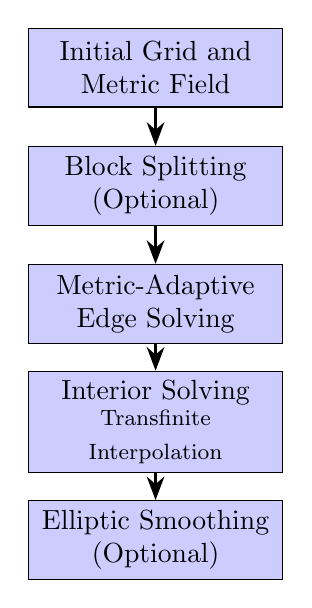
\begin{tikzpicture}[
    node distance=1.5cm,
    box/.style={rectangle, draw, fill=blue!20, text width=3cm, align=center, minimum height=1cm},
    arrow/.style={-{Stealth[length=3mm]}, thick}
  ]
    \node[box] (tfi) {Initial Grid and Metric Field};
    \node[box, below of=tfi] (split) {Block Splitting\\(Optional)};
    \node[box, below of=split] (edge) {Metric-Adaptive\\Edge Solving};
    \node[box, below of=edge] (interior) {Interior Solving\\\footnotesize{Transfinite}\\\footnotesize{Interpolation}};
    \node[box, below of=interior] (smooth) {Elliptic Smoothing\\(Optional)};
    
    \draw[arrow] (tfi) -- (split);
    \draw[arrow] (split) -- (edge);
    \draw[arrow] (edge) -- (interior);
    \draw[arrow] (interior) -- (smooth);
  \end{tikzpicture}
  \end{center}
\end{frame}

\begin{frame}{Input Format Overview}
  \textbf{Required Inputs:}
  \begin{itemize}
    \item \texttt{initialGrid}: Tortuga-style grid 
    \begin{itemize}
      \item Array of grid blocks containing node coordinates
      \item Array of block boundary conditions
      \item Array of interface between blocks
    \end{itemize}
    \item \texttt{M}: Riemannian Metric Tensor field
    \begin{itemize}
      \item Array of 2D metric tensors at each grid node
      \item A custom metric can be designed if no residual-based metric is available.
    \end{itemize}
  \end{itemize}
  \textbf{Optional Inputs:}
  \begin{itemize}
    \item \texttt{params}: User Defined Simulation Parameters
  \end{itemize}
  \vspace{0.5cm}
  \textbf{Note:}
  \begin{itemize}
    \item Grid Adaptation compared to Generation from Scratch
  \end{itemize}
\end{frame}

\begin{frame}{Block Splitting}
\begin{itemize}
  \item Block splits allow for more control over the grid structure. 
  \item GridGeneration.jl does not support full multi-block capability \textit{yet}.
  \item Block splits are all 1-1 node connections which may be merged at the end back together.
  \item New block numbers, interfaces and boundaries are automatically generated during splitting.
  \item Format: \texttt{splitIndices = [[i\_splits],[j\_splits]]}
    \begin{itemize}
      \item \texttt{i\_splits}: Array of i-indices to split along j-direction
      \item \texttt{j\_splits}: Array of j-indices to split along i-direction
    \end{itemize}
\end{itemize}
\end{frame}

\begin{frame}{Block Splitting Example}
\begin{figure}[]
  \centering
  \includegraphics[width=\textwidth,height=\textwidth,keepaspectratio]{images/block-split.png}
  \caption{initial and split grid shown in left and right respectively using user defined splits: \texttt{splitIndices = [[300, 500],[40]]}} 
  \label{fig}
\end{figure}
\end{frame}

% ============================================================================
\section{1D Formulation of 2D Grid Generation}
% ============================================================================

\begin{frame}
  \begin{center}
    {\Large 1D Formulation of 2D Grid Generation}
  \end{center}
\end{frame}

\begin{frame}{Problem Statement}
    \begin{columns}
    \column{0.5\textwidth}
    \textbf{Input:} A 2D metric tensor field $M$ and a domain $\Omega$ with edges $\Gamma_i$, $i=1,2,3,4$.

    \vspace{0.5cm}
    \textbf{Output:} A mesh $\mathcal{T}$ of $\Omega$ such that the distribution and number of points along the boundaries $\Gamma_i$ agrees with the metric $M$.

    \vspace{0.5cm}
    \textbf{Needed:} A way to represent $M$ and $\Gamma_i$ in 1D. For now, assume such exists.
    
    \column{0.5\textwidth}
    \begin{center}
    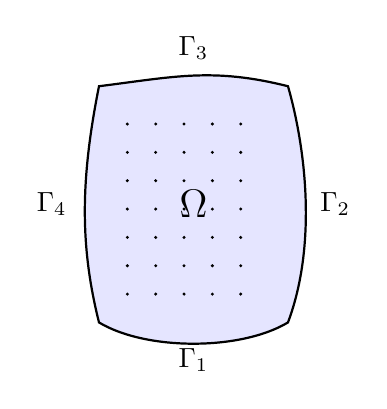
\begin{tikzpicture}[scale=1.2]
      % Define the domain with curved sides
      \draw[thick, fill=blue!10] 
        (0,0) coordinate (BL) 
        .. controls (0.5,-0.3) and (1.5,-0.3) .. 
        (2,0) coordinate (BR)
        .. controls (2.3,0.8) and (2.2,1.8) ..
        (2,2.5) coordinate (TR)
        .. controls (1.2,2.7) and (0.8,2.6) ..
        (0,2.5) coordinate (TL)
        .. controls (-0.2,1.5) and (-0.2,0.8) ..
        cycle;
      
      % Label the interior
      \node at (1,1.25) {\Large $\Omega$};
      
      % Label the edges
      \node at (1,-0.4) {$\Gamma_1$};
      \node at (2.5,1.25) {$\Gamma_2$};
      \node at (1,2.9) {$\Gamma_3$};
      \node at (-0.5,1.25) {$\Gamma_4$};
      
      % Add some grid points to suggest mesh
      \foreach \x in {0.3,0.6,...,1.8} {
        \foreach \y in {0.3,0.6,...,2.2} {
          \fill (\x,\y) circle (0.5pt);
        }
      }
    \end{tikzpicture}
    \end{center}
    \end{columns}
\end{frame}

\begin{frame}{ODE Formulation}
    Let $s$ denote the computational domain $[0,1]$, $x(s)$ the physical domain, $\sigma$ is the element-spacing, and $m(x(s))$ the (1D) metric tensor field. We define the loss function as
    
    \[L_\text{misfit}(x_s, x, s) = m^2; \quad m(x_s, x, s) = \sigma^2  M x_s^2 - 1.\]

    We will use variable subscripts to denote derivatives $\left( x_s := \frac{dx}{ds} \right)$. 
\end{frame}

\begin{frame}{Optimal Distribution - Euler-Lagrange}
    To compute $\mathcal{T}$, we aim to minimizing the functional
    
    \[ \mathcal{L}[x(s)] = \int_{\Omega_i} L_\text{misfit}(x_s, x, s) ds. \]
    
    The optimal solution $x(s)$ satisfies the Euler-Lagrange equation

    \[\frac{\partial L_\text{misfit}}{\partial x} -  \frac{d}{ds} \left( \frac{\partial L_\text{misfit}}{\partial x_s} \right) = 0, \]

    Solving the above ODE will give the optimal distribution mapping from computational to physical space along edge $\Gamma_i$.
    
\end{frame}

\begin{frame}{Euler-Lagrange (Cont.)}
    We can compute the partials to be
    \begin{align*}
        \frac{\partial L_\text{misfit}}{\partial x} &= 2 \sigma^2 m M_x x_s^2, \\
        \frac{\partial m}{\partial s} &= \sigma^2 (M_x x_s^3 + 2 M x_s x_{ss}), \\
        \frac{\partial L_\text{misfit}}{\partial x_s} &=  4 \sigma^2 m M x_s, \\
        - \frac{d}{ds} \left( \frac{\partial L_\text{misfit}}{\partial x_s} \right) &= - 4 \sigma^2 (m_s M x_s + m M_x x_s^2 + m M x_{ss}).
    \end{align*}
    Plugging everything into the Euler-Lagrange equation, we get
    \begin{align*}
        \frac{\partial L}{\partial x} -  \frac{d}{ds} \left( \frac{\partial L}{\partial x_s} \right) &= -  8 \sigma^4 M^2 x_s^2 x_{ss} - 4 \sigma^4 M M_x x_s^4 \\ &\quad\quad - 4 \sigma^2 m M x_{ss} - 2 \sigma^2 m M_x x_{s}^2 = 0.  
    \end{align*}
\end{frame}


\begin{frame}{2nd Order ODE Simplification}
    We aim to solve the 2nd order ODE
    \begin{align*}
        -  8 \sigma^4 M^2 x_s^2 x_{ss} - 4 \sigma^4 M M_x x_s^4 - 4 \sigma^2 m M x_{ss} - 2 \sigma^2 m M_x x_{s}^2 = 0.  
    \end{align*}
    Dividing both sides by $-2 \sigma^2$ (as $\sigma \neq 0$), 
    \begin{align*}
        4 \sigma^2 M^2 x_s^2 x_{ss} + 2 \sigma^2 M M_x x_s^4 + 2 m M x_{ss} + m M_x x_{s}^2 = 0,\\
        \iff (4 \sigma^2 M^2 x_s^2  + 2 m M) x_{ss}  = - (2 \sigma^2 M M_x x_s^4+ m M_x x_{s}^2).
    \end{align*}
    Solving for $x_{ss}$ yields
    \begin{align*}
        x_{ss} &= - \frac{2 \sigma^2 M M_x x_s^4+ m M_x x_{s}^2}{4 \sigma^2 M^2 x_s^2  + 2 m M},
        = - \frac{ x_s^2 M_x (2 \sigma^2 M x_s^2 + m )}{2M (2 \sigma^2 M x_s^2  +  m )},
    \end{align*}
    Therefore
    \[ 
      \boxed{x_{ss} = - \frac{M_x}{2M} x_s^2.}
    \]
\end{frame}


\begin{frame}{Optimal Number of Points}
    We additionally require 
    \begin{equation*}
        \frac{\partial L_\text{misfit}}{\partial \sigma} = 0,
    \end{equation*}
    which gives the optimal number of points along the boundary $\Gamma$. We can compute
    \begin{equation*}
        \sigma = \sqrt{ \frac{\int_{\hat{\Omega}} p d V}{\int_{\hat{\Omega}} p^2 d V} }; \quad p = M x_s^2.
    \end{equation*}
    The optimal number of points along $\Gamma_i$ is then given by $N_i = \frac{1}{\sigma}$.
\end{frame}



\begin{frame}{Final ODE System}
    Finally, we can rewrite the problem now along edge $\Gamma_i$ with arc length $L_i$ as: 

    \textbf{Distribution:}
    \begin{equation}\label{eq:ode-dist}
        x_{ss} = - \frac{M_x}{2M} x_s^2; \quad x(s=0) = 0, \quad x(s=1) = L_i.
    \end{equation}

    \textbf{Number of Points:}
    \begin{equation}\label{eq:ode-numpts}
        \sigma = \sqrt{ \frac{\int_{\hat{\Omega}} M x_s^2 d V}{\int_{\hat{\Omega}} (M x_s^2)^2 d V} }.
    \end{equation}

    Note that \eqref{eq:ode-numpts} can be computed after solving \eqref{eq:ode-dist} using trapezoidal rule. We then resolve \eqref{eq:ode-dist} using the optimal $\sigma$.  
\end{frame}

\begin{frame}{Analytic Solution}
    The semi-analytic solution to \eqref{eq:ode-dist} can by derived by noting that
    \begin{equation*}
        \frac{d M}{d s} = \frac{d M}{d x} \frac{d x}{d s} = M_x x_s,  
    \end{equation*}
    which gives
    \begin{equation*}
        x_{ss} = - \frac{M_x}{2M} x_s^2 = - \frac{M_s}{2M} x_s.
    \end{equation*}
    Now assuming that $x_s \neq 0$ \footnote{okay since $x_s = 0 \iff x = \text{const}$ which wouldn't be a valid mapping of $x(s)$.}, we can divide both sides by $x_s$ to get
    \begin{equation*}
        \frac{x_{ss}}{x_s} = - \frac{M_s}{2M}, \implies  \ln x_s  = -  \frac{C}{2} \ln M,
    \end{equation*}
    where $C$ is a constant of integration. Thus we have that
    \begin{equation*}\label{eq:xs}
        x_s = C M^{-\frac{1}{2}}
    \end{equation*}
    
\end{frame}

\begin{frame}{Analytic Solution Continued}
    Rearranging terms yields
    \begin{equation*}
        M^{\frac{1}{2}} dx = C ds \implies \int_0^{x} M^{\frac{1}{2}}(\xi) d\xi = C \int_0^s ds = Cs.
    \end{equation*}
    Noting that $x(0) = 0$ it trivially satisfied, we can solve for $C$ using the boundary condition $x(1) = L_i$ to get
    \begin{equation*}
        C = \int_0^{L_i} M^{\frac{1}{2}}(\xi) d\xi,
    \end{equation*}
    and so the analytic solution to \eqref{eq:ode-dist} is given by the implicit equation
    \begin{equation*}
        \int_0^{x} M^{\frac{1}{2}}(\xi) d\xi = s \int_0^{L_i} M^{\frac{1}{2}}(\xi) d\xi.
    \end{equation*}
    or if we let $I(x) = \int_0^x M^{\frac{1}{2}}(\xi) d\xi$, then
    \begin{equation*}
        I(x) = I(L_i) s \implies x = I^{-1}(I(L_i) s),
    \end{equation*}
    
\end{frame}


\begin{frame}{Analytic Solution - Numerical Inverision}
To compute $x(s)$ numerically we will use that since $\sqrt{M} > 0$, $I(x)$ is strictly increasing and so invertible
\[
\int_0^{x(s)} \sqrt{M(\xi)} \, d\xi = s \int_0^1 \sqrt{M(\xi)} \, d\xi,
\quad s \in [0,1].
\]

Step 1. Discretize the cumulative integral.
\[
I_k \;\approx\; \int_0^{x_k} \sqrt{M(\xi)} \, d\xi, 
\qquad
I_{k+1} = I_k + \tfrac{1}{2}\,(w_k + w_{k+1})(x_{k+1}-x_k),
\]
where $w_i = \sqrt{M(x_i)}$.

Step 2. Uniform $s$-grid and target values.
\[
s_j = \frac{j}{N}, 
\qquad
t_j = s_j \, I_{\text{tot}}, 
\qquad I_{\text{tot}} = I_n.
\]

Step 3. Invert $I(x)$ by linear interpolation.
Find $i$ with $I_i \le t_j \le I_{i+1}$, then
\[
x_j \;\approx\; x_i + \theta (x_{i+1} - x_i),
\qquad
\theta = \frac{t_j - I_i}{I_{i+1}-I_i}.
\]
\end{frame}

\begin{frame}{Verification - Example 1}
    \begin{figure}[H]
        \centering
        \includegraphics[width=0.8\textwidth,height=\textwidth,keepaspectratio]{images/1d_verification_problem1.png}
        \caption{$M = k^2$ with $L=5$, $k=200$, and $N=100$.}
    \end{figure}   
\end{frame}

\begin{frame}{Verification - Example 2}
    \begin{figure}[H]
        \centering
        \includegraphics[width=0.8\textwidth,height=\textwidth,keepaspectratio]{images/1d_verification_problem2.png}
        \caption{$M = (a + bx)^2$ with $L=5$, $a=5$, $b=5$, and $N=100$.}
    \end{figure}   
\end{frame} 

\begin{frame}{Verification - Example 3}
    \begin{figure}[H]
        \centering
        \includegraphics[width=0.8\textwidth,height=\textwidth,keepaspectratio]{images/1d_verification_problem3.png}
        \caption{$M = s(1 + 15(x))^{-2}$ with $L=1$, $s=40000$, and $N=100$.}
    \end{figure}   
\end{frame} 

\begin{frame}{Verification - Example 4}
    \begin{figure}[H]
        \centering
        \includegraphics[width=0.8\textwidth,height=\textwidth,keepaspectratio]{images/1d_verification_problem4.png}
        \caption{$M = s(1 + 15(x))^{-2} + s(1 + 15(1 - x))^{-2}$ with $L=1$, $s=40000$, and $N=100$.}
    \end{figure}   
\end{frame} 

\begin{frame}
  \begin{center}
    {\Large How Do we Map the 2D Domain and Metric to Match the 1D Formulation?}
  \end{center}
\end{frame}

\begin{frame}{2D Extension - Metric Tensor Projection}
    \textbf{To find a 1D representation, $m$, of the 2D tensor $M$:} 
    Suppose $\Gamma_i$ is discretized with points $\left\{\gamma_j \right\}_{j=1}^N$ with $N$ points. Let's use a central difference like method to compute $m_j$ at each point $\gamma_j$ along $\Gamma_i$. We approximate using
    {\small 
    \begin{equation*}
        m_j := \frac{1}{|\gamma_{j+1} - \gamma_{j-1}|^2}(\gamma_{j+1} - \gamma_{j-1})^\top \cdot  \begin{pmatrix} M_{11} & M_{12} \\ M_{21} & M_{22} \end{pmatrix}_j \cdot (\gamma_{j+1} - \gamma_{j-1}), j=2,\cdots, N - 1,
    \end{equation*} 
    }
    and a one-sided like approximation for the endpoints
    $$
    m_1 := \frac{1}{|\gamma_{2} - \gamma_{1}|^2}(\gamma_{2} - \gamma_{1})^\top  \cdot \begin{pmatrix} M_{11} & M_{12} \\ M_{21} & M_{22} \end{pmatrix}_1 \cdot (\gamma_{2} - \gamma_{1}),
    $$

    $$
    m_N := \frac{1}{|\gamma_{N} - \gamma_{N-1}|^2}(\gamma_{N} - \gamma_{N-1})^\top \cdot \begin{pmatrix} M_{11} & M_{12} \\ M_{21} & M_{22} \end{pmatrix}_N \cdot (\gamma_{N} - \gamma_{N-1}).
    $$

    \textbf{Note:} Since $M$ is positive definite, $m_j > 0$ for all $j$ by construction.
\end{frame}

\begin{frame}{Metric Tensor Projection - Visualization}
    \begin{center}
    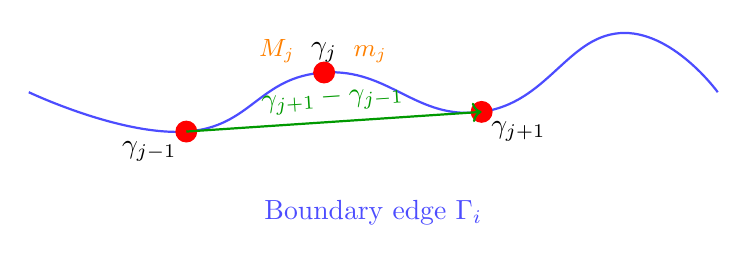
\begin{tikzpicture}[scale=2.5]
      % Draw a curved boundary edge
      \draw[thick, blue!70] plot[smooth, tension=0.8] coordinates {
        (0,0.5) (0.8,0.3) (1.5,0.6) (2.3,0.4) (3,0.8) (3.5,0.5)
      };
      
      % Mark three consecutive points
      \coordinate (p1) at (0.8,0.3);
      \coordinate (p2) at (1.5,0.6);
      \coordinate (p3) at (2.3,0.4);
      
      % Draw points
      \filldraw[red] (p1) circle (1.5pt);
      \filldraw[red] (p2) circle (1.5pt);
      \filldraw[red] (p3) circle (1.5pt);
      
      % Draw tangent vectors (difference vectors)
      \draw[->, thick, green!60!black] (p1) -- (p3) node[midway, above, sloped] {$\gamma_{j+1} - \gamma_{j-1}$};
      
      % Label points
      \node[below left] at (p1) {$\gamma_{j-1}$};
      \node[above] at (p2) {$\gamma_j$};
      \node[below right] at (p3) {$\gamma_{j+1}$};
      
      % Add edge label
      \node[below, blue!70] at (1.75, 0) {Boundary edge $\Gamma_i$};
      
      % % Draw metric tensor representation at middle point
      % \draw[thick, orange, ->] (p2) -- ++(0.3, 0.2) node[right] {\small $M_j$};
      \node[above left, orange] at (1.4,0.6) {\small $M_j$};
      \node[above right, orange] at (1.6,0.6) {\small $m_j$};
      
    \end{tikzpicture}
    \end{center}
    
    \vspace{0.3cm}
    The metric projection uses the direction vector $(\gamma_{j+1} - \gamma_{j-1})$ to compute the 1D metric $m_j$ from the 2D tensor $M_j$ at point $\gamma_j$.
\end{frame}

\begin{frame}{1D Metric Example 1}
    \begin{figure}[H]
        \centering
        \includegraphics[width=0.8\textwidth,height=\textwidth,keepaspectratio]{images/1dmetric-ex1.png}
        \caption{2D Metric Tensor $M$ (top) and Projected 1D Metric $m$ (bottom) along boundary $\Gamma_i$.}
    \end{figure}
\end{frame}


\begin{frame}{2D Extension - Boundary Projection}
    We can then project the 2D points $\gamma_i = (x_i, y_i)$ to a 1D domain using the spacing between points. Let $\eta_i$ be the 1D projected points, where $\eta_1 = 0$ and
    \begin{equation*}
        \eta_i = \sum_{j=2}^{i-1} |\gamma_{j+1} - \gamma_{j}|, \quad i=2,\cdots,N.
    \end{equation*}
    We note that $\eta_N = |\Gamma_1|$.
\end{frame}

\begin{frame}{Boundary Projection - Visualization}
    \begin{center}
    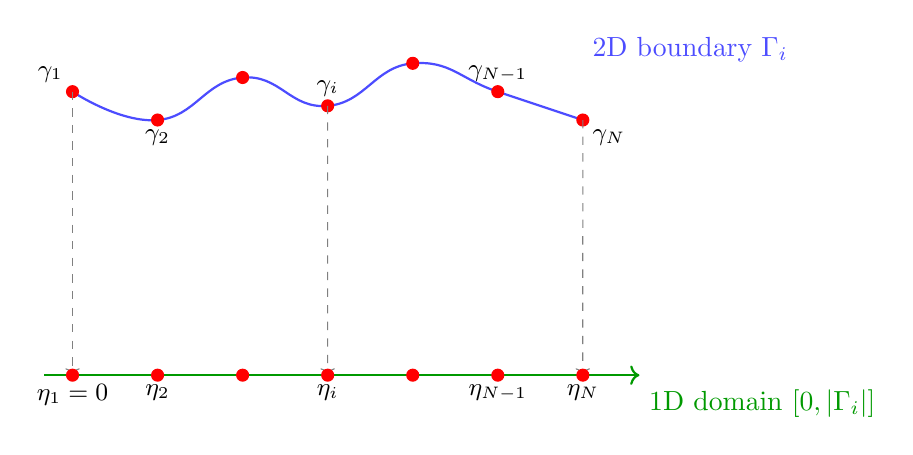
\begin{tikzpicture}[scale=1.8]
      % Draw a curved boundary edge (2D)
      \draw[thick, blue!70] plot[smooth, tension=0.8] coordinates {
        (0,2.5) (0.6,2.3) (1.2,2.6) (1.8,2.4) (2.4,2.7) (3.0,2.5) (3.6,2.3)
      };
      
      % Mark points on the curve
      \coordinate (g1) at (0,2.5);
      \coordinate (g2) at (0.6,2.3);
      \coordinate (g3) at (1.2,2.6);
      \coordinate (g4) at (1.8,2.4);
      \coordinate (g5) at (2.4,2.7);
      \coordinate (g6) at (3.0,2.5);
      \coordinate (g7) at (3.6,2.3);
      
      % Draw points on curve
      \foreach \i in {1,2,3,4,5,6,7} {
        \filldraw[red] (g\i) circle (1.2pt);
      }
      
      % Label some points on curve
      \node[above left] at (g1) {\small $\gamma_1$};
      \node[below] at (g2) {\small $\gamma_2$};
      \node[above] at (g4) {\small $\gamma_i$};
      \node[above] at (g6) {\small $\gamma_{N-1}$};
      \node[below right] at (g7) {\small $\gamma_N$};
      
      % Add edge label
      \node[right, blue!70] at (3.6, 2.8) {2D boundary $\Gamma_i$};
      
      % Draw projection arrows
      \draw[->, dashed, gray] (g1) -- (0,0.5);
      \draw[->, dashed, gray] (g4) -- (1.8,0.5);
      \draw[->, dashed, gray] (g7) -- (3.6,0.5);
      
      % Draw 1D line
      \draw[thick, green!60!black, ->] (-0.2,0.5) -- (4.0,0.5);
      
      % Mark points on 1D line
      \coordinate (e1) at (0,0.5);
      \coordinate (e2) at (0.6,0.5);
      \coordinate (e3) at (1.2,0.5);
      \coordinate (e4) at (1.8,0.5);
      \coordinate (e5) at (2.4,0.5);
      \coordinate (e6) at (3.0,0.5);
      \coordinate (e7) at (3.6,0.5);
      
      % Draw points on line
      \foreach \i in {1,2,3,4,5,6,7} {
        \filldraw[red] (e\i) circle (1.2pt);
      }
      
      % Label points on line
      \node[below] at (e1) {\small $\eta_1=0$};
      \node[below] at (e2) {\small $\eta_2$};
      \node[below] at (e4) {\small $\eta_i$};
      \node[below] at (e6) {\small $\eta_{N-1}$};
      \node[below] at (e7) {\small $\eta_N$};
      
      % Add 1D domain label
      \node[right, green!60!black] at (4.0, 0.3) {1D domain $[0, |\Gamma_i|]$};
      
    \end{tikzpicture}
    \end{center}
    
    \vspace{0.2cm}
    The projection maps 2D boundary points $\gamma_i$ to 1D coordinates $\eta_i$ by accumulating arc lengths between consecutive points.
\end{frame}

\begin{frame}{2D Extension - Solving the 1D Problem}
    We can now solve the 1D problem using the projected metric tensor and boundary points on the domain $[0, |\Gamma_1|]$. We use $f_i = \frac{(m_x)_i}{2 m_i}$, where $(m_x)_i$ is approximated using the central difference scheme and solve
    \begin{equation*}
        \eta_{ss} = - f(\eta) \eta_s^2; \quad \eta(s=0) = 0, \quad \eta(s=1) = \eta_N = |\Gamma_1|.
    \end{equation*}
    We can then compute the optimal number of points along $\Gamma_1$ using
    \begin{equation*}
        \sigma = \sqrt{ \frac{\int_{0}^{1} m(\eta) \eta_s^2 d s}{\int_{0}^{1} (m(\eta) \eta_s^2)^2 d s} }.
    \end{equation*}
\end{frame}

\begin{frame}{2D Extension - Mapping Back to 2D}
    We can then map the 1D solution back to 2D using linear interpolation:

    Step 1. Interval identification.
\[
\text{Find } j \ \text{such that } \eta_i^* \in [\gamma_j,\, \gamma_{j+1}],
\]
where $\{\gamma_j\}$ is the boundary discretization.

Step 2. Normal distance computation from $\gamma_j$.
\[
d_i = \frac{|\eta_i^* - \gamma_j|}{|\gamma_{j+1} - \gamma_j|}.
\]

Step 3. Projection onto boundary.
\[
\gamma_i^* = d_i \gamma_{j+1} + (1 - d_i) \gamma_j.
\]

\end{frame}

\begin{frame}{Mapping Back to 2D - Visualization}
    \begin{center}
    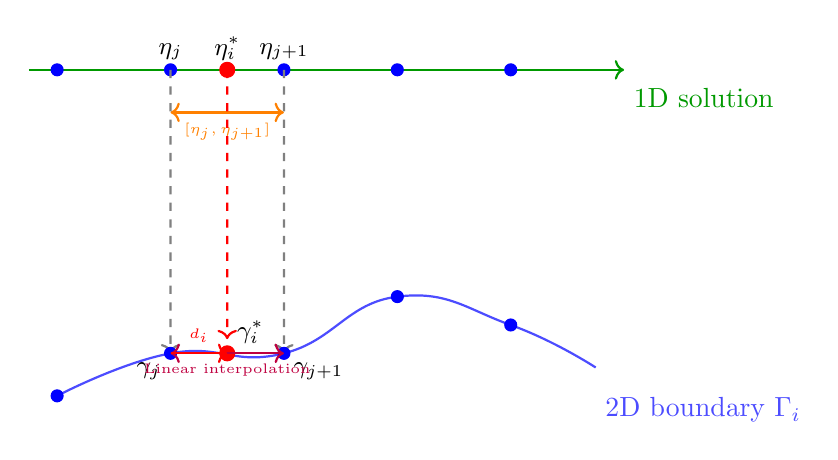
\begin{tikzpicture}[scale=1.8]
      % Draw 1D line at top
      \draw[thick, green!60!black, ->] (-0.2,2.8) -- (4.0,2.8);
      
      % Mark original points on 1D line
      \coordinate (e1) at (0,2.8);
      \coordinate (e2) at (0.8,2.8);
      \coordinate (e3) at (1.6,2.8);
      \coordinate (e4) at (2.4,2.8);
      \coordinate (e5) at (3.2,2.8);
      
      % Draw original points
      \foreach \i in {1,2,3,4,5} {
        \filldraw[blue] (e\i) circle (1.2pt);
      }
      
      % Mark new optimal point on 1D line
      \coordinate (eNew) at (1.2,2.8);
      \filldraw[red] (eNew) circle (1.5pt);
      
      % Label points on 1D line
      \node[above] at (e2) {\small $\eta_j$};
      \node[above] at (eNew) {\small $\eta_i^*$};
      \node[above] at (e3) {\small $\eta_{j+1}$};
      
      % Add 1D domain label
      \node[right, green!60!black] at (4.0, 2.6) {1D solution};
      
      % Draw interval highlight
      \draw[thick, orange, <->] (0.8,2.5) -- (1.6,2.5) node[midway, below] {\tiny $[\eta_j, \eta_{j+1}]$};
      
      % Draw projection arrows
      \draw[->, dashed, gray, thick] (e2) -- (0.8,0.8);
      \draw[->, dashed, red, thick] (eNew) -- (1.2,0.9);
      \draw[->, dashed, gray, thick] (e3) -- (1.6,0.8);
      
      % Draw a curved boundary edge (2D)
      \draw[thick, blue!70] plot[smooth, tension=0.8] coordinates {
        (0,0.5) (0.8,0.8) (1.6,0.8) (2.4,1.2) (3.2,1.0) (3.8,0.7)
      };
      
      % Mark points on curve corresponding to original 1D points
      \coordinate (g1) at (0,0.5);
      \coordinate (g2) at (0.8,0.8);
      \coordinate (g3) at (1.6,0.8);
      \coordinate (g4) at (2.4,1.2);
      \coordinate (g5) at (3.2,1.0);
      
      % Draw original boundary points
      \foreach \i in {1,2,3,4,5} {
        \filldraw[blue] (g\i) circle (1.2pt);
      }
      
      % Mark the interpolated new point on curve
      \coordinate (gNew) at (1.2,0.8);
      \filldraw[red] (gNew) circle (1.5pt);
      
      % Label points on curve
      \node[below left] at (g2) {\small $\gamma_j$};
      \node[above right] at (gNew) {\small $\gamma_i^*$};
      \node[below right] at (g3) {\small $\gamma_{j+1}$};
      
      % Draw interpolation segment
      \draw[thick, purple, <->] (g2) -- (g3) node[midway, below, sloped] {\tiny Linear interpolation};
      
      % Add distance marker
      \draw[thick, red, ->] (g2) -- (gNew) node[midway, above] {\tiny $d_i$};
      
      % Add edge label
      \node[right, blue!70] at (3.8, 0.4) {2D boundary $\Gamma_i$};
      
    \end{tikzpicture}
    \end{center}
    
    \vspace{0.2cm}
    The optimal 1D point $\eta_i^*$ is mapped back to the 2D boundary by finding the interval $[\eta_j, \eta_{j+1}]$ it falls in, then linearly interpolating between $\gamma_j$ and $\gamma_{j+1}$.
\end{frame}

\begin{frame}{Metric-Adaptive Edge Solving Procedure}
  \textbf{Algorithm Overview:} Solve edges for a single block with metric field $M$
  
  \vspace{0.2cm}
  {\small
  \begin{algorithmic}[1]
    \STATE \textbf{Input:} Block with edges $\{\Gamma_1, \Gamma_2, \Gamma_3, \Gamma_4\}$, metric field $M$
    \FOR{each edge $\Gamma_i$ with points $\{\gamma_j\}$}
      \STATE Compute 1D metric: $m_j$
      \STATE Project to 1D: $\eta_j$
    \ENDFOR
    \FOR{each edge $\Gamma_i$}
      \STATE Solve ODE $x(s)$ using projected $m$ and $\eta$
      \STATE Compute optimal spacing $\sigma_i$
      \STATE Compute number of points: $N_i \leftarrow \lceil 1/\sigma_i \rceil$
    \ENDFOR
    \STATE \textbf{// Enforce matching opposite edges}
    \STATE $N_\text{horiz} \leftarrow \max(N_1, N_3)$ \hfill \textit{// Bottom and top}
    \STATE $N_\text{vert} \leftarrow \max(N_2, N_4)$ \hfill \textit{// Right and left}
    \STATE \textbf{// Resolve with fixed number of points}
    \STATE Resolve $\Gamma_1, \Gamma_3$ with $N_\text{horiz}$ points
    \STATE Resolve $\Gamma_2, \Gamma_4$ with $N_\text{vert}$ points
    \STATE Map 1D solutions back to 2D
    \STATE \textbf{Output:} Optimally distributed edge points
  \end{algorithmic}
  }
\end{frame}

\begin{frame}{Not True Block Splitting}
  Since GridGeneration.jl only supports multi-block grids with matching interfaces, this means that the number of points along opposite edges must match not only within a block, but also across blocks. Thus, we modify the above procedure to account for multiple blocks:
  
  \vspace{0.3cm}
  \begin{center}
  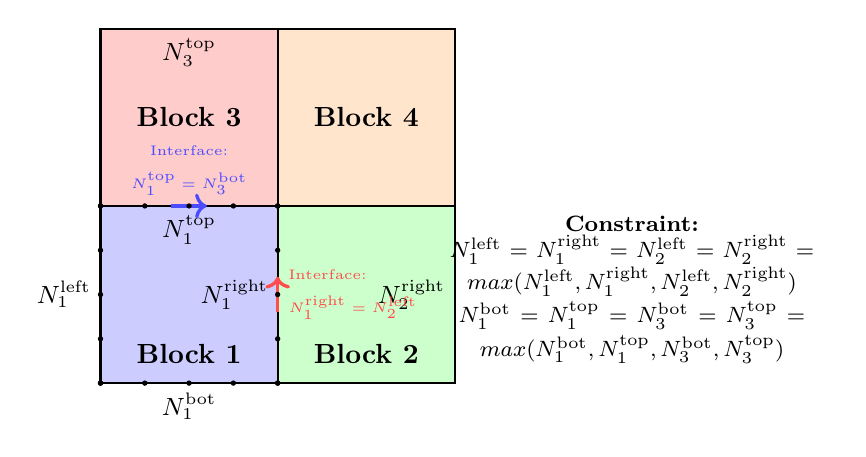
\begin{tikzpicture}[scale=1.5]
    % Draw the four blocks
    \draw[thick, fill=blue!20] (0,0) rectangle (1.5,1.5);
    \draw[thick, fill=green!20] (1.5,0) rectangle (3,1.5);
    \draw[thick, fill=red!20] (0,1.5) rectangle (1.5,3);
    \draw[thick, fill=orange!20] (1.5,1.5) rectangle (3,3);
    
    % Label the blocks
    \node at (0.75,0.25) {\textbf{Block 1}};
    \node at (2.25,0.25) {\textbf{Block 2}};
    \node at (0.75,2.25) {\textbf{Block 3}};
    \node at (2.25,2.25) {\textbf{Block 4}};
    
    % Add edge labels with N values for Block 1
    \node[below] at (0.75,0) {\small $N_1^{\text{bot}}$};
    \node[left] at (1.5,0.75) {\small $N_1^{\text{right}}$};
    \node[below] at (0.75,1.5) {\small $N_1^{\text{top}}$};
    \node[left] at (0,0.75) {\small $N_1^{\text{left}}$};
    
    \node[left] at (3,0.75) {\small $N_2^{\text{right}}$};
    \node[below] at (0.75, 3) {\small $N_3^{\text{top}}$};

    % Draw arrows showing propagation
    % Horizontal propagation (left-right edges)
    \draw[->, very thick, red!70] (1.5,0.6) -- (1.5,0.9) 
      node[midway, right, align=left] {\tiny Interface:\\ \tiny $N_1^{\text{right}} = N_2^{\text{left}}$};
    
    % Vertical propagation (top-bottom edges)
    \draw[->, very thick, blue!70] (0.6,1.5) -- (0.9,1.5) 
      node[midway, above, align=center] {\tiny Interface:\\ \tiny $N_1^{\text{top}} = N_3^{\text{bot}}$};
    
    % Add constraint indicators
    \node[below, align=center, text width=5cm] at (4.5,1.5) {
      \footnotesize \textbf{Constraint:} \\$N_1^{\text{left}} = N_1^{\text{right}} = N_2^{\text{left}} = N_2^{\text{right}} = max(N_1^{\text{left}}, N_1^{\text{right}}, N_2^{\text{left}}, N_2^{\text{right}})$\\
      \footnotesize $N_1^{\text{bot}} = N_1^{\text{top}} = N_3^{\text{bot}} = N_3^{\text{top}} = max(N_1^{\text{bot}}, N_1^{\text{top}}, N_3^{\text{bot}}, N_3^{\text{top}})$
    };
    
    % Add small dots to represent grid points on edges
    \foreach \x in {0, 0.375, 0.75, 1.125, 1.5} {
      \filldraw[black] (\x,0) circle (0.5pt);
      \filldraw[black] (\x,1.5) circle (0.5pt);
    }
    \foreach \y in {0, 0.375, 0.75, 1.125, 1.5} {
      \filldraw[black] (0,\y) circle (0.5pt);
      \filldraw[black] (1.5,\y) circle (0.5pt);
    }
    
  \end{tikzpicture}
  \end{center}
  
  \vspace{0.2cm}
\end{frame}

\begin{frame}{Core Workflow}
  \begin{center}
  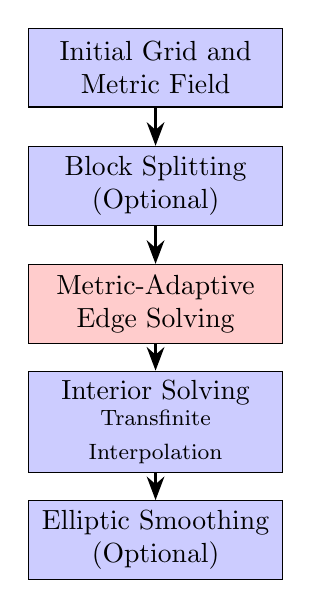
\begin{tikzpicture}[
    node distance=1.5cm,
    box/.style={rectangle, draw, fill=blue!20, text width=3cm, align=center, minimum height=1cm},
    boxc/.style={rectangle, draw, fill=red!20, text width=3cm, align=center, minimum height=1cm},
    arrow/.style={-{Stealth[length=3mm]}, thick}
  ]
    \node[box] (tfi) {Initial Grid and Metric Field};
    \node[box, below of=tfi] (split) {Block Splitting\\(Optional)};
    \node[boxc, below of=split] (edge) {Metric-Adaptive\\Edge Solving};
    \node[box, below of=edge] (interior) {Interior Solving\\\footnotesize{Transfinite}\\\footnotesize{Interpolation}};
    \node[box, below of=interior] (smooth) {Elliptic Smoothing\\(Optional)};
    
    \draw[arrow] (tfi) -- (split);
    \draw[arrow] (split) -- (edge);
    \draw[arrow] (edge) -- (interior);
    \draw[arrow] (interior) -- (smooth);
  \end{tikzpicture}
  \end{center}
\end{frame}

\begin{frame}{Interior Solving - Transfinite Interpolation}
    After solving the edges, we can compute the interior points using transfinite interpolation (TFI) for each block. For a block with edges $\Gamma_1, \Gamma_2, \Gamma_3, \Gamma_4$, we can compute the interior points using
    \begin{equation*}
        x(\xi, \eta) = (1 - \eta) x_{\Gamma_1}(\xi) + \eta x_{\Gamma_3}(\xi) + (1 - \xi) x_{\Gamma_4}(\eta) + \xi x_{\Gamma_2}(\eta) - \text{correction\_terms},
    \end{equation*}
    where the correction terms account for double counting at the corners. This is a 2D extension of linear interpolation.

    \vspace{0.3cm}
    \textbf{Note:} TFI is very fast but can lead to poor quality grids, especially for highly skewed or curved boundaries.
\end{frame}

\begin{frame}{Custom Metric}
\small
\textbf{Goal:} Define a spatially varying isotropic metric
\[
M(x,y) = \begin{bmatrix} w(x,y) & 0 \\ 0 & w(x,y) \end{bmatrix},
\qquad w(x,y) > 0,
\]
to control point clustering near the boundary and a user defined hotspot.

Weight function:
\[
w(x,y) = \underbrace{w_{\text{rational}}\!\bigl(d_{\text{airfoil}}(x,y)\bigr)}_{\text{distance to boundary}}
+ \underbrace{w_{\text{rational}}\!\bigl(d_{\text{hotspot}}(x,y)\bigr)}_{\text{distance to hotspot}}
+ w_{\min}.
\]

Profiles:
\[
w_{\text{rational}}(d;A,\ell,p) = \frac{A}{1 + (d/\ell)^p}.
\]

\textbf{Parameters:}
\begin{itemize}
  \item $A$ = amplitude (strength of clustering),
  \item $\ell$ = decay length,
  \item $p$ = tail sharpness,
  \item $w_{\min}$ = positive floor far from features.
\end{itemize}
\end{frame}

\begin{frame}{Grid Adaptation Gif}
    Pull up the gif here:

    \url{https://www.marvyn.com/GridGeneration.jl/stable/pages/SingleBlock/nosplitting/}

    \vspace{0.3cm}

    \textbf{Observations:}
    \begin{itemize}
        \item Points cluster near the airfoil boundary due to the distance-based metric
        \item Additional clustering occurs around the hotspot, demonstrating metric adaptability
        \item But the grid has poor quality (such as angle skewness) near the airfoil surface due to TFI
        \item In worst cases, TFI can lead to interior points leaving the domain
        \item To improve quality, 
        \begin{itemize}
          \item Can try to use more interior block splitting
          \item Use TFI as initial guess for elliptic and variational methods which take mesh quality into account. Talk more about this later.
        \end{itemize} 
    \end{itemize}
\end{frame}
\begin{frame}{Core Workflow}
  \begin{center}
  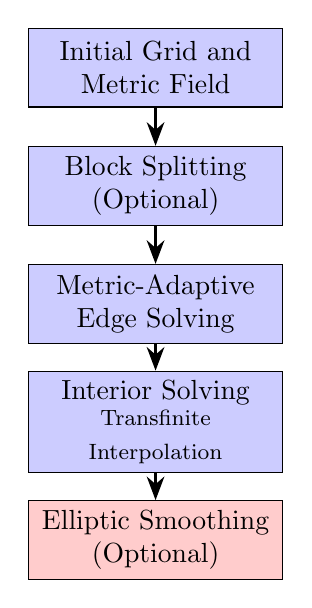
\begin{tikzpicture}[
    node distance=1.5cm,
    box/.style={rectangle, draw, fill=blue!20, text width=3cm, align=center, minimum height=1cm},
    boxc/.style={rectangle, draw, fill=red!20, text width=3cm, align=center, minimum height=1cm},
    arrow/.style={-{Stealth[length=3mm]}, thick}
  ]
    \node[box] (tfi) {Initial Grid and Metric Field};
    \node[box, below of=tfi] (split) {Block Splitting\\(Optional)};
    \node[box, below of=split] (edge) {Metric-Adaptive\\Edge Solving};
    \node[box, below of=edge] (interior) {Interior Solving\\\footnotesize{Transfinite}\\\footnotesize{Interpolation}};
    \node[boxc, below of=interior] (smooth) {Elliptic Smoothing\\(Optional)};
    
    \draw[arrow] (tfi) -- (split);
    \draw[arrow] (split) -- (edge);
    \draw[arrow] (edge) -- (interior);
    \draw[arrow] (interior) -- (smooth);
  \end{tikzpicture}
  \end{center}
\end{frame}

\begin{frame}{Smoothing Methods}
  \textbf{To Improve Mesh quality:}
  \begin{itemize}
    \item \textbf{Hyperbolic Generation:} Rather than filling in the interior using TFI, let's use a hyperbolic marching method with smoothing terms to propagate the boundary points. Note that the outer domain here can not be specified. Use this method to fill in points near the boundary, then extend to outer domain using TFI or other methods.
    \item \textbf{Elliptic Grid Generation:}\footnote{Only method currently implemented in GridGeneration.jl} Solve a set of coupled Poisson equations to smooth the grid while controlling orthogonality and spacing near boundaries.
    \item \textbf{Variational Methods:} Minimize an energy functional that penalizes poor quality elements, leading to a more uniform and well-shaped grid.
  \end{itemize}
\end{frame}

\begin{frame}{Elliptic Grid Generation - Poisson Equations}
    Let $(x,y)$ denote the physical domain and $(\xi, \eta)$ the computational domain. We solve the following two Poisson equations for $\xi(x,y)$ and $\eta(x,y)$:
    \begin{align*}
        \xi_{xx} + \xi_{yy} &= P(\xi,\eta),\\
        \eta_{xx} + \eta_{yy} &= Q(\xi,\eta),
    \end{align*}
    where $P$ and $Q$ are forcing terms that control the orthogonality and smoothness of the grid. After some calculations, we can rewrite the equations in terms of the physical domain as
    \begin{align*}
        \alpha x_{\xi\xi} - 2 \beta x_{\xi\eta} + \gamma x_{\eta\eta} &= - J^{2}(P x_\xi + Q x_\eta),\\
        \alpha y_{\xi\xi} - 2 \beta y_{\xi\eta} + \gamma y_{\eta\eta} &= - J^{2}(P y_\xi + Q y_\eta),
    \end{align*}
    where $\alpha = x_\eta^2 + y_\eta^2$, $\beta = x_\xi x_\eta + y_\xi y_\eta$, $\gamma = x_\xi^2 + y_\xi^2$, and $J = x_\xi y_\eta - x_\eta y_\xi$ (the Jacobian of the transformation).
\end{frame}

\begin{frame}{Elliptic Grid Generation - Forcing Terms}
    To understand the forcing terms $P$ and $Q$, let's focus on the boundary along $\eta_1$. To ensure a smooth decay into the interior, we use exponential decay functions
    \begin{align*}
        P = P_0 e^{-a(\eta - \eta_1)}, \quad Q = Q_0 e^{-b(\eta - \eta_1)},
    \end{align*}
    where $a,b > 0$ are decay rates. The terms $P_0$ and $Q_0$ are solved for to ensure orthogonality along the boundary $\eta_1$ and a desired grid spacing of $s$.
\end{frame} 

\begin{frame}{Elliptic Grid Generation - Forcing Terms (Cont.)}
    To solve for $P_0$ and $Q_0$, we note that orthogonality along $\eta_1$ requires that
    \begin{equation*}
        x_\xi x_\eta + y_\xi y_\eta = 0 \implies \beta = 0.
    \end{equation*}
    We also want to ensure that the grid spacing along $\eta_1$ is $s$. This can be achieved by enforcing
    \begin{equation*}
        \sqrt{x_\eta^2 + y_\eta^2} = s \implies \alpha = s^2.
    \end{equation*}
    Using these two conditions, we can solve for $x_\eta$ and $y_\eta$ to find:
    \begin{align*}
        \left. x_\eta \right|_{\eta=\eta_{1}}= - \frac{s y_\xi}{\sqrt{x_\xi^2 + y_\xi^2}}, \quad \left. y_\eta \right|_{\eta=\eta_{1}} = \frac{s x_\xi}{\sqrt{x_\xi^2 + y_\xi^2}}.
    \end{align*}
    We can also compute $x_{\eta\eta}$ and $y_{\eta\eta}$ along $\eta_1$ using a taylor expansion:
    \begin{align*}
        \left. x_{\eta\eta} \right|_{\eta=\eta_{1}} &= \frac{1}{2}(-7x_1 + 8 x_2 - x_3) - 3 \left. x_{\eta} \right|_{\eta=\eta_{1}}\\
        \left. y_{\eta\eta} \right|_{\eta=\eta_{1}} &= \frac{1}{2}(-7y_1 + 8 y_2 - y_3) - 3 \left. y_{\eta} \right|_{\eta=\eta_{1}}.
    \end{align*}
\end{frame}

\begin{frame}{Elliptic Grid Generation - Forcing Terms (Cont.)}
    Plugging these into the Poisson equations along $\eta_1$ gives
    \begin{align*}
        P_0(\xi, \eta_1) &= J^{-1} \left( y_\eta R_1 - x_\eta R_2 \right),\\
        Q_0(\xi, \eta_1) &= J^{-1} \left( y_\xi R_1 + x_\xi R_2 \right),
    \end{align*}
    where
    \begin{align*}
        R_1 &= -J^{-2}(\alpha x_{\xi\xi} -2\beta x_{\xi\eta} + \gamma x_{\eta\eta}),\\
        R_2 &= -J^{-2}(\alpha y_{\xi\xi} -2\beta y_{\xi\eta} + \gamma y_{\eta\eta}).
    \end{align*}
    
\end{frame}

\begin{frame}{Post Processing Tools}
    \textbf{Angle Deviation from Orthogonality:}
    For each grid point $(i,j)$, compute the vector to neighbors $(i,j+1)$ and $(i+1,j)$, denoted $\vec{e}_1$ and $\vec{e}_2$, and compute the angle between them: 
    \begin{equation*}
        \theta = \arccos\left(\frac{\vec{e}_1 \cdot \vec{e}_2}{|\vec{e}_1||\vec{e}_2|}\right)
    \end{equation*}
    Then the deviation from orthogonality is $|\theta - 90^\circ|$.
\end{frame}

\begin{frame}{Post Processing Tools - Example}
    \begin{figure}[H]
        \centering
        \includegraphics[width=\textwidth,height=\textwidth,keepaspectratio]{images/a_angle_deviation_case_4.pdf}
    \end{figure}
\end{frame}

\begin{frame}
  \begin{center}
    {\Large Using GridGeneration.jl}
  \end{center}
\end{frame}

\begin{frame}{Installing Julia}
  \textbf{Step 1: Install Julia}
  
  \vspace{0.3cm}
  \begin{itemize}
    \item Go to the official Julia website: \url{https://julialang.org/downloads/}
    \item Download the latest stable version for your operating system (Windows, macOS, Linux).
    \item Follow the installation instructions specific to your OS.
  \end{itemize}
  
  \vspace{0.5cm}
  \textbf{Step 2: Verify Installation}
  
  \vspace{0.3cm}
  \begin{itemize}
    \item Open a terminal or command prompt.
    \item Type `julia` and press Enter.
    \item You should see the Julia REPL 
  \end{itemize}
\end{frame}

\begin{frame}{Installing GridGeneration.jl}
  \textbf{Step 1: Open Julia REPL}
  
  \vspace{0.3cm}
  \begin{itemize}
    \item Open your terminal or command prompt.
    \item Type `julia` and press Enter to start the Julia REPL.
  \end{itemize}
  
  \vspace{0.5cm}
  \textbf{Step 2: Import Pkg Module}

  \vspace{0.3cm}
  \begin{itemize}
    \item In the Julia REPL, type `using Pkg` and press Enter.
  \end{itemize}

  \vspace{0.5cm}
  \textbf{Step 3: Install GridGeneration.jl}
  \vspace{0.3cm}
  \begin{itemize}
    \item Type `Pkg.add("GridGeneration")` and press Enter.
    \item Wait for the installation to complete.
  \end{itemize}
\end{frame}

\begin{frame}{Example of Pipeline}
  An example of the entire pipeline can be found in examples/generalExample\_blank.jl
\end{frame}

\begin{frame}{Using GridGenerationGUI.jl}
  I thought it would be fun to put together an interactive GUI for GridGeneration.jl using Makie.jl. This allows users to visualize and interactively modify grid generation parameters and see the results in real-time. The parameters can be saved to a Julia script for later use.
\end{frame}


\begin{frame}{Summary}
  \textbf{GridGeneration.jl provides:}
  
  \begin{itemize}
    \item \textbf{Efficient} metric-based grid generation
    \item \textbf{Flexible} multi-block support with automatic propagation
    \item \textbf{Modular} design for different use cases
    \item \textbf{Quality} Various Smooth Methods to enhance grid quality
  \end{itemize}
  
  \vspace{0.5cm}
  \begin{block}{Core Idea}
    Transforms 2D grid generation into tractable 1D ODE problems, enabling efficient metric-based adaptation while maintaining structured grid properties
  \end{block}
  
  \vspace{0.5cm}
  \textbf{GitHub:} \url{https://github.com/marvynbailly/GridGeneration.jl}

  \textbf{Documentation:} \url{https://marvyn.com/GridGeneration.jl/dev/}
\end{frame}

\begin{frame}
  \begin{center}
    {\Huge Thank You!}
    
    \vspace{1cm}
    {\Large Questions?}
  \end{center}
\end{frame}

\end{document}
